

\section{SOFTWARE DEVELOPMENT METHODOLOGY}
\subsection{Software Development Life Cycle}
A software development methodology or system development methodology is a framework that is used to structure, plan, and control the process of developing a software system. It is the practice of using selected process techniques to improve the quality of a software development effort. The documented collection of policies, processes and procedures used by a development team or organization to practice software engineering is called its software development methodology (SDM) or system development life cycle (SDLC). For the timely and successful implementation of any project one must follow a suitable software development model. For the purpose of our project we followed an incremental software building model as our project consists of several functional components to be developed in a incremental manner. In incremental model, the whole requirement is divided into various builds. During each iteration, the development module goes through the requirements, design, implementation and testing phases. Each subsequent release of the module adds function to the previous release. The process continues till the complete system is ready as per the requirement. It starts with a simple implementation of a subset of the software requirements and iteratively enhances the evolving versions until the full system is implemented. At each iteration, design modifications are made and new functional capabilities are added. The basic idea behind this method is to develop a system through repeated cycles  and in smaller portions at a time.
\begin{figure}[h]
	\begin{center}
		
		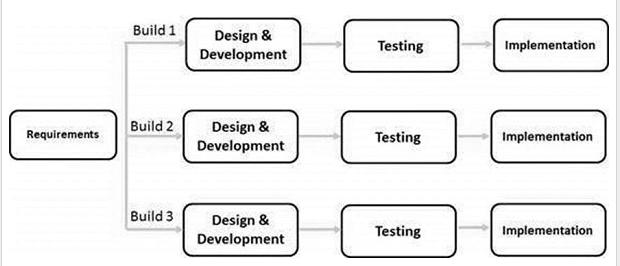
\includegraphics[scale=0.6]{SDLC.png}
		\caption{An Incremental Approach for Software Development}
		\label{SDLC}
	\end{center}
\end{figure}

Some of the basic characteristics of this software development methodology are:
\begin{itemize}
	\item Major requirements are defined; however, some functionalities or requested enhancements may evolve with time.
	\item Some working functionality can be developed quickly and early in the life cycle.
	\item Results are obtained early and periodically.
	\item Parallel development can be planned.
	\item Less costly to change the scope/requirements.
	\item Risk analysis is better and it supports changing requirements.
	\item Partial systems are built to produce the final system.
\end{itemize}

By following this model, we focused on building several components of the system in an incremental basis and finally those components are merged together to form a total functional system of Interactive voice response system with speech recognition module.


\subsection{Requirement Analysis}
Requirements analysis, also called requirements engineering, is the process of determining user expectations for a new system that is going to be build. These features, called requirements, must be quantifiable, relevant and detailed. In software engineering, such requirements are often called functional specifications. Requirements analysis is an important aspect of project management.
Requirements analysis involves frequent communication with system users to determine specific feature expectations, resolution of conflict or ambiguity in requirements as demanded by the various users or groups of users, avoidance of feature creep and documentation of all aspects of the project development process from start to finish. Energy should be directed towards ensuring that the final system or product conforms to client needs rather than attempting to mold user expectations to fit the requirements. Requirements analysis is a team effort that demands a combination of hardware, software and human factors engineering expertise as well as skills in dealing with people.

\subsubsection{Functional Requirements}

Functional requirements explain what has to be done by identifying the necessary task, action or activity that must be accomplished. In our project the core functional requirements can be as depicted in below:
\begin{enumerate}
	\item The system must be able to classify a voice signal from an independent speaker.
	\item The system must involve a significant degree of user interaction.
	\item The system must be able to run on different cross platforms.
	\item The system should allow the real time voice input by the user.
	\item The system must be capable of removing the potential noise effects on input voice signal
	
\end{enumerate}

\subsubsection{Non-Functional Requirements}
Non-functional requirements are requirements that specify criteria that can be used to judge the operation of a system, rather than specific behaviors. The non-functional requirements of the project  are listed below:

\begin{enumerate}
	\item The training of the sound samples must be effective and efficient.
	\item Mechanism of training sample generation must be easy and fast.
	\item The integration of all the system modules that compose a system must be easier and effective.
	\item The feedback from the system must be quick and in real time to make user feel in control during the interaction.
	
	
	
\end{enumerate}


\subsection{Feasibility Study}
Speech Recognition is one of the hottest topic in the current field of technology and science. Many researches have been carried out in this field from several decades ago to till today and many of them are still under study to optimize the study. The ASR system have been utilized in several sectors and have proved their importance in today\textquotesingle s technological world. By undertaking this project our attempt is to make use of speech recognition in a simple interactive system to automate the task using the voice command. We have undergone through several feasibility studies to make sure that the project is feasible and be developed . Some study topics are discussed below:


\subsubsection{Technical Feasibility}
ASR have been utilized under several platforms and several development approaches have been developed. Development of new artificial intelligence and pattern matching models have made it more simpler for implementation of ASR embedded with interactive system. Similarly today\textquotesingle s powerful computing processors and easy data collection software makes it more technically feasible.
\subsubsection{Operational Feasibility}
Many researches have been carried out in the field interactive systems using ASR most of which using English language. Such systems have proved to be easily operable several platforms. Our project is just a kind of implementation of ASR to automate task through Nepali voice . Thus this makes it operationally feasible for development.
\subsubsection{Economic Feasibility}
The project is economically feasible to begin with as no expensive hardware and software components is required. Similarly all the tools and techniques to be used are open source and are easily available free of cost. Data collection is done among us and other individuals which is economically feasible.
\subsubsection{Schedule  Feasibility}
To develop the project a proper time line has been projected to complete relevant portion of the project in scheduled time period. Most of the Necessary resources are  searched on the web and are available to begin research in time. Also all the related software packages are easily available which makes if more feasible.

\subsection{System Design}
\subsubsection{Use Case Diagram}

\begin{figure}[H]
	\begin{center}
		
		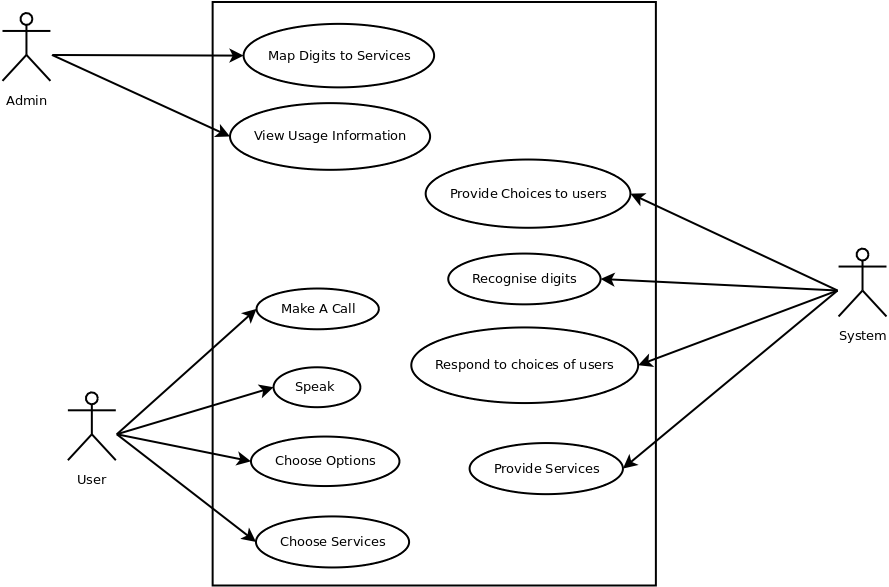
\includegraphics[width = \linewidth]{Usecase}
		\caption{Use Case Diagram}
	\end{center}
\end{figure}
\subsubsection{Sequence Diagram}
\begin{figure}[H]
	\begin{center}
		
		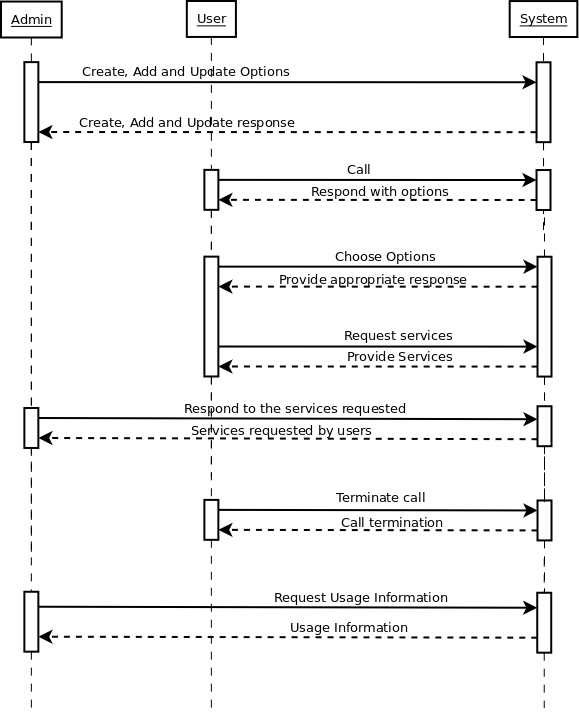
\includegraphics[scale = 0.5]{sequence}
		\caption{Sequence Diagram}
	\end{center}
\end{figure}

\subsubsection{Data Flow Diagram}
\begin{figure}[H]
	\begin{center}
		
		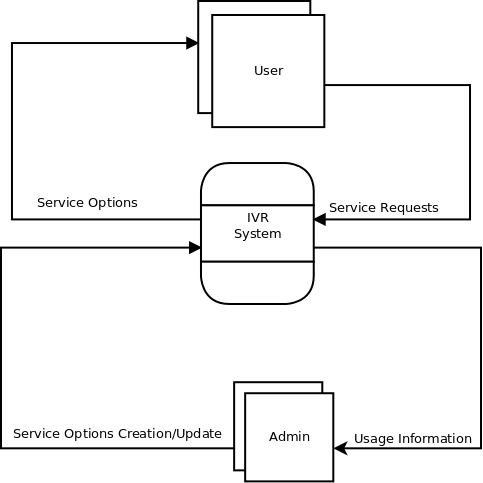
\includegraphics[scale = 0.5]{DFD}
		\caption{Data Flow Diagram}
	\end{center}
\end{figure}
\subsection{Tools and Technologies}
\subsubsection{Python Programming Language}
Python is a general-purpose, open source computer programming language. It is optimized for software quality, developer productivity, program portability, and component integration. Python is used by at least hundreds of thousands of developers around the world in areas such as internet scripting, systems programming, user interfaces, product customization, numeric programming, and more. It is generally considered to be among the top four or five most widely-used programming languages in the world today.

As a popular language focused on shrinking development time, python is deployed in
a wide variety of products and roles. Counted among its current user base are Google,
YouTube, industrial light and magic, esri, the bit torrent file sharing system, NASA\textquotesingle s
jet propulsion lab, the game eve online, and the national weather service. Python\textquotesingle s
application domains range from system administration, website development, cell
phone scripting, and education to hardware testing, investment analysis, computer games, and spacecraft control. Among other things, python sports a remarkably simple, readable, and maintainable syntax; integration with external components coded in other languages; a multiparadigm design, with OOP, functional, and modular structures; and a vast collection of precoded interfaces and utilities. Its tool set makes it a flexible and agile language,
ideal for both quick tactical tasks as well as longer-range strategic application development efforts. Python features a dynamic type system and automatic memory management and supports multiprogramming paradigms including object oriented, imperative, functional programming, and procedural styles. It has a large and comprehensive standard library. Python interpreters are available for many operating systems, allowing Python code to run on a wide variety of systems. Although it is a general-purpose language, python is often called a scripting language because it makes it easy to utilize and direct other software components. Perhaps python\textquotesingle s best asset, though, is simply that it makes software development more rapid and enjoyable. 

The major reasons behind the use of python programming language for this project are discussed below in brief.
\begin{itemize}
	\item Software quality:
	
	For many, Python\textquotesingle s focus on readability, coherence, and software quality in general
	sets it apart from other tools in the scripting world. Python code is designed to be
	readable, and hence reusable and maintainable much more so than traditional
	scripting languages. The uniformity of Python code makes it easy to understand,
	even if you did not write it. In addition, Python has deep support for more advanced
	software reuse mechanisms, such as object-oriented programming (OOP) and function programming.
	
	\item Developer productivity:
	
	Python boosts developer productivity many times beyond compiled or statically
	typed languages such as C, C++, and Java. Python code is typically one-third to
	one-fifth the size of equivalent C++ or Java code. That means there is less to type, 
	less to debug, and less to maintain after the fact. Python programs also run immediately, without the lengthy compile and link steps required by some other tools, 
	further boosting programmer speed.
	
	\item Program Portability:
	
	Most Python programs run unchanged on all major computer platforms. Porting
	Python code between Linux and Windows, for example, is usually just a matter of
	copying a script\textquotesingle s code between machines. Moreover, Python offers multiple options for coding portable graphical user interfaces, database access programs, web based systems, and more. Even operating system interfaces, including program launches and directory processing are as portable is Python as they can possibly be.
	
	\item Support Libraries:
	
	Python comes with a large collection of pre-built and portable functionality, known
	as the standard library. This library supports an array of application-level programming tasks, from text pattern matching to network scripting. In addition,
	Python can be extended with both homegrown libraries and a vast collection of
	third-party application support software. Python \textquotesingle s third-party domain offers tools
	for website construction, numeric programming, serial port access, game development, and much . The NumPy extension, for instance, has been described as a free and more powerful equivalent to the Matlab numeric programming system.
	
	\item Component Integration:
	
	Python scripts can easily communicate with other parts of an application, using a
	variety of integration mechanisms. Such integrations allow Python to be used as a
	product customization and extension tool. Today, Python code can invoke C and
	C++ libraries, can be called from C and C++ programs, can integrate with Java
	and .NET components, can communicate over frameworks such as COM and Silverlight, can interface with devices over serial ports, and can interact over networks
	with interfaces like SOAP, XML-RPC, and CORBA. It is not a standalone tool.
\end{itemize}
\subsubsection{NumPy}
NumPy is the high performance numeric programming extension for python. It is the core library for scientific computing in Python. It is a Python library that provides a multidimensional array object, various derived objects (such as masked arrays and matrices), and an assortment of routines for fast operations on arrays, including mathematical, logical, shape manipulation, sorting, selecting, I/O, discrete Fourier transforms, basic linear algebra, basic statistical operations, random simulation and much more.

It contains among other things:

\begin{itemize}
	\item a powerful N-dimensional array object
	\item sophisticated (broadcasting) functions
	\item tools for integrating C/C++ and Fortran code
	\item useful linear algebra, Fourier transform, and random number capabilities
\end{itemize}

Besides its obvious scientific uses, NumPy can also be used as an efficient multi-dimensional container of generic data. Arbitrary data-types can be defined. This allows NumPy to seamlessly and speedily integrate with a wide variety of databases.
\subsubsection{PyAudio}
PyAudio provides Python bindings for PortAudio, the cross-platform audio I/O library. With PyAudio, you can easily use Python to play and record audio on a variety of platforms. PyAudio is inspired by:

\begin{itemize}
	\item pyPortAudio/fastaudio: Python bindings for PortAudio v18 API.
	\item tkSnack: cross-platform sound toolkit for Tcl/Tk and Python.
\end{itemize}

PyAudio provides Python bindings for PortAudio, the cross-platform audio I/O library. With PyAudio, you can easily use Python to play and record audio on a variety of platforms. PyAudio is inspired by:
pyPortAudio/fastaudio: Python bindings for PortAudio v18 API.
tkSnack: cross-platform sound toolkit for Tcl/Tk and Python.
To use PyAudio, we first instantiate PyAudio using pyaudio.PyAudio() , which sets up the portaudio system. To record or play audio, we open a stream on the desired device with the desired audio parameters using pyaudio.PyAudio.open() . This sets up a pyaudio.Stream to play or record audio.  We play audio by writing audio data to the stream using pyaudio.Stream.write(), or read audio data from the stream using pyaudio.Stream.read().
In "blocking mode" each pyaudio.Stream.write() or pyaudio.Stream.read() blocks until all the given/requested frames have been played/recorded. Alternatively, to generate audio data on the fly or immediately process recorded audio data, use the "callback mode". 

\subsubsection{Pomegranate}
pomegranate is a python package which implements fast, efficient, and extremely flexible
probabilistic models ranging from probability distributions to Bayesian networks to
mixtures of hidden Markov models. Pomegranate has been used in our project to create the
HMM models.	
\subsubsection{PyQT}
PyQt4 is a toolkit for creating GUI applications. It is a blending of Python programming language and the successful Qt library. Qt library is one of the most powerful GUI libraries. PyQt4 is developed by Riverbank Computing. 

PyQt4 is implemented as a set of Python modules. It has 440 classes and 6000 functions and methods. It is a multiplatform toolkit which runs on all major operating systems, including UNIX, Windows, and Mac OS. PyQt4 is dual licensed. Developers can choose between a GPL and a commercial license. Previously, GPL version was available only on UNIX. Starting from PyQt version 4, GPL license is available on all supported platforms.


PyQt4's classes are divided into several modules. Some of them are:
\begin{itemize}
	\item QtCore
	\item QtGui
	\item QtNetwork
	\item QtXml
	\item QtSvg
	\item QtOpenGL
	\item QtSql
\end{itemize}
The QtCore module contains the core non GUI functionality. This module is used for working with time, files and directories, various data types, streams, URLs, mime types, threads or processes. The QtGui module contains the graphical components and related classes. These include for example buttons, windows, status bars, toolbars, sliders, bitmaps, colours, and fonts. The QtNetwork module contains the classes for network programming. These classes facilitate the coding of TCP/IP and UDP clients and servers by making the network programming easier and more portable. The QtXmlcontains classes for working with XML files. This module provides implementation for both SAX and DOM APIs. The QtSvg module provides classes for displaying the contents of SVG files. Scalable Vector Graphics (SVG) is a language for describing two-dimensional graphics and graphical applications in XML. The QtOpenGL module is used for rendering 3D and 2D graphics using the OpenGL library. The module enables seamless integration of the Qt GUI library and the OpenGL library. The QtSql module provides classes for working with databases.

\subsubsection{TensorFlow}

TensorFlow is an open source software library for numerical computation using data flow graphs. Nodes in the graph represent mathematical operations, while the graph edges represent the multidimensional data arrays (tensors) communicated between them. The flexible architecture allows us to deploy computation to one or more CPUs or GPUs in a desktop, server, or mobile device with a single API. TensorFlow was originally developed by researchers and engineers working on the Google Brain Team within Google's Machine Intelligence research organization for the purposes of conducting machine learning and deep neural networks research, but the system is general enough to be applicable in a wide variety of other domains as well. 

\subsubsection{keras}

Keras is a high-level neural networks API, written in Python and capable of running on top of TensorFlow, CNTK, or Theano. It enables  fast experimentation.

\subsection{Project Scheduling}

\begin{figure}[H]
	\begin{center}
		
		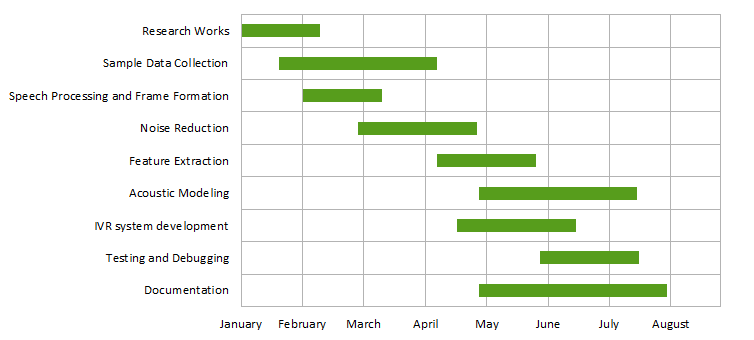
\includegraphics[width = \linewidth]{gantt}
		\caption{Gantt Chart for Project}
	\end{center}
\end{figure}
